\documentclass{beamer}

\usepackage{blindtext}
\usepackage{tcolorbox}
\usepackage{listings}
\lstset{
	frame=tb,                        % = tb to put top and bottom
	framerule=0pt,
	framextopmargin=3pt,
	framexbottommargin=3pt,
	basicstyle=\small\ttfamily,      % the size of the fonts that are used for the code
	backgroundcolor=\color{gray!10},
	numbers=none,                    % where to put the line-numbers; possible values are (none, left, right)
	stringstyle=\color{black},       % string literal style
}

\usetheme{Patorikku}

\title{Konobi game}
\subtitle{Software Development Method Project}
\author{Fallacara E., Indri P., Pigozzi F.}
\date{}


\begin{document}
  % Per decidere se mostrare il numero di slide oppure no.
	\setcounter{showSlideNumbers}{0}

  % Pagina di titolo.
	\frame{\titlepage}

  % Azzera il contatore dei frame e inizia a mostrarlo.
	\setcounter{framenumber}{0}
	\setcounter{showSlideNumbers}{1}

  
%\section{Introduction and rules}

  \begin{frame}{Introduction}

    \begin{tcolorbox}[colback=red!90!black!10]
      The \textbf{goal} of our project is to implement the \textbf{Konobi game} in Java, giving also the user the opportunity to choose between two interfaces: \textbf{console version} or \textbf{GUI version}.
    \end{tcolorbox}

    \vspace{1em}

    \begin{block}{Tools}
      \begin{itemize}
        \item IntelliJ;
        \item OpenJDK11 and JavaFX;
        \item GitHub;
        \item Gradle: building;
        \item TravisCI: continuous integrations;
        \item \textcolor{red}{Other?}
      \end{itemize}
    \end{block}

  \end{frame}


\section{Konobi Game}

  \begin{frame}{Konobi}

    Konobi is a drawless connection game for two players: \textbf{Black}
    and \textbf{White}. It's played on the a square board, which is initially empty. 

    \vspace{1em}

    The top and bottom edges of the board are coloured black; the left and right edges are coloured white.

    \vspace{1em}

    \begin{centering}

      \fcolorbox{black}{yellow!70!black!40}{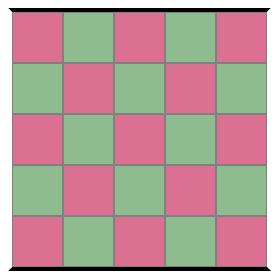
\includegraphics[width=0.35\textwidth]{img/empty.png}}

    \end{centering}

  \end{frame}



  \begin{frame}{Konobi Rules}

    \textbf{Starting with Black}, the players take turns placing stones of their own color on empty points of the board, one stone per turn.\pause

    \vspace{1em}

    Two like-coloured stones are \textbf{strongly connected} if they are orthogonally adjacent to each other, and \textbf{weakly connected} if they are diagonally adjacent to each other without sharing any strongly connected neighbour.\pause

    \vspace{1em}

    It's \textbf{illegal} to make a weak connection to a certain stone unless it's impossible to make a placement which is both strongly connected to that stone and not weakly connected to another.

  \end{frame}


  \begin{frame}{Legal and Illegal Moves}

    \begin{centering}

      Legal moves:

      \vspace{1em}

      \fcolorbox{black}{yellow!70!black!40}{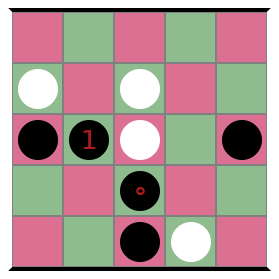
\includegraphics[width=0.25\textwidth]{img/legal1.png}}\hspace{0.1\textwidth}
      \fcolorbox{black}{yellow!70!black!40}{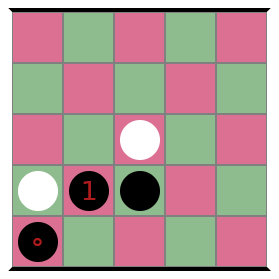
\includegraphics[width=0.25\textwidth]{img/legal2.png}}\pause

      \vspace{1em}

      Illegal moves:

      \vspace{1em}

      \fcolorbox{black}{yellow!70!black!40}{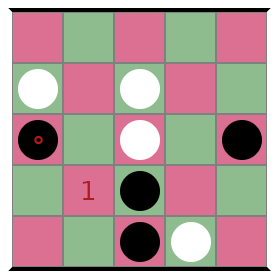
\includegraphics[width=0.25\textwidth]{img/illegal1.png}}\hspace{0.1\textwidth}%
      \fcolorbox{black}{yellow!70!black!40}{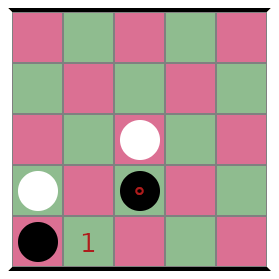
\includegraphics[width=0.25\textwidth]{img/illegal2.png}}\par

    \end{centering}


  \end{frame}



  \begin{frame}{Konobi rules Cont.}

    It's also \textbf{illegal} to form a \textbf{crosscut}, i.e., a 2x2 pattern of stones consisting of two weakly connected Black stones and two weakly connected White stones.

    \vspace{1em}

    \begin{centering}

      \fcolorbox{black}{yellow!70!black!40}{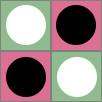
\includegraphics[width=0.25\textwidth]{img/cross.png}}

    \end{centering}\pause

    \vspace{1em}

    If a player can't make a move on his turn, he must \textbf{pass}. Passing is otherwise not allowed. There will always be a move available to at least one of the players.

  \end{frame}


  \begin{frame}{Konobi rules Cont.}

    The \textbf{pie rule} is used in order to make the game fair. This means that White will have the option, on his first turn only, to change sides instead of making a regular move.\pause

    \vspace{3em}

    The game is \textbf{won} by the player who completes a chain of his color touching the two opposite board edges of his color. \textbf{Draws are not possible}.

  \end{frame}


 \section{Project Structure}

  \begin{frame}{Project Structure} 
  The project is subdivided in two main packages:
    \begin{itemize}
        \item \textcolor{red}{core}
        \item \textcolor{red}{user interface}
     \end{itemize}

 \vspace{4em}

	
    \end{frame}

 \begin{frame}{Project  Strcuture}
  The project is subdivided in two main packages:
  \begin{itemize}
        \item \textcolor{red}{core}
        \item \textcolor{red}{user interface}
   \end{itemize}

 \vspace{1em}

  The \textbf{core package}  contains all the elements concerning the functional logic of the game.

 \vspace{2em}

	
 \end{frame}

 \begin{frame}{Project  Strcuture}
  The project is subdivided in two main packages:
  \begin{itemize}
        \item \textcolor{red}{core}
        \item \textcolor{red}{user interface}
   \end{itemize}

 \vspace{1em}

  The \textbf{core package}  contains all the elements concerning the functional logic of the game.

 \vspace{1em}

 The \textbf{UI package}, on the other hand, contains all the elements that are used to create the two different user interfaces: \textbf{command line} and \textbf{desktop interface}.
	
 \end{frame}



\section{Core Package}

  \begin{frame}{Building Blocks}

    \textbf{Cell} class is the fundamental building block of the game engine. It is associated to a \textbf{Colour}, and has a \textbf{Point} for the coordinates.

    \vspace{1em}

    \textbf{Board} class is a collection of \textbf{Cell}s, and implements the \textbf{Iterable} interface. It conveys a notion of geometrical arrangement among the \textbf{Cell}s.

    \vspace{1em}

    \textbf{Player} class represents each of the two players.

    \end{frame}


    \begin{frame}{Building Blocks - TDD}

    \begin{centering}

     \fcolorbox{black}{yellow!70!black!40}{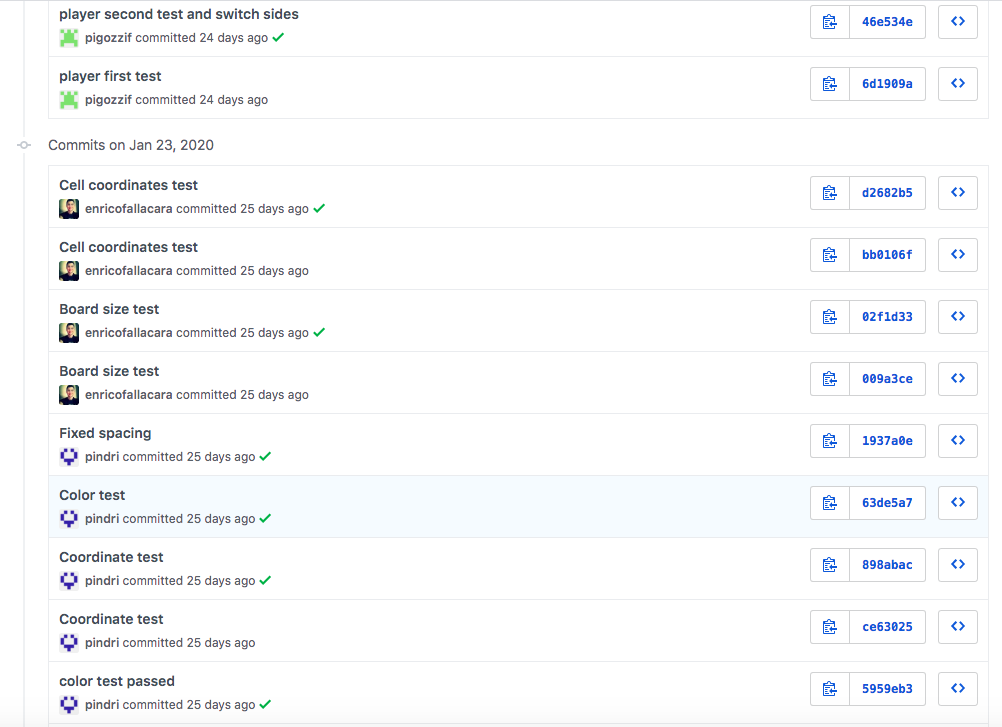
\includegraphics[width=0.75\textwidth]{img/TDD.png}}

     \end{centering}

     \vspace{1em}

     \textbf{Test Driven Development} was adopted from the very onset, committing after every red-light/green-light pattern.

     \end{frame}


     \begin{frame}{SRP and Board}

     {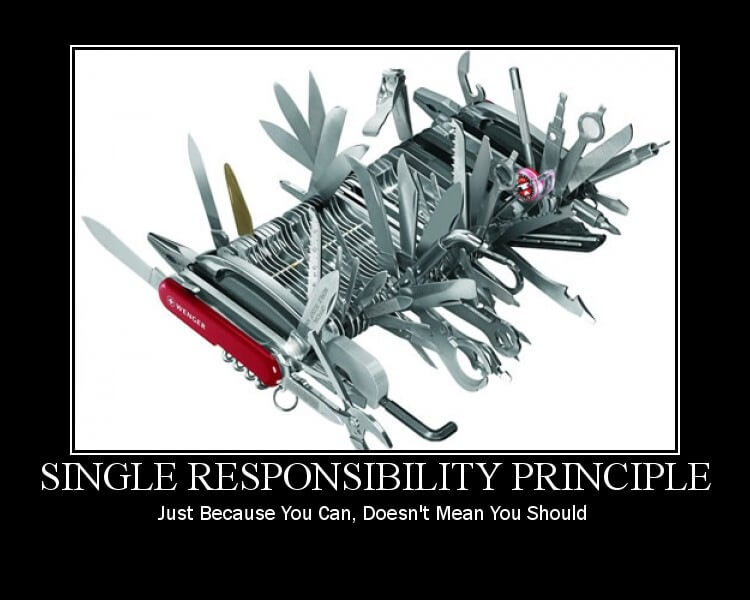
\includegraphics[width=0.45\textwidth]{img/singleresponsibilityprinciple.jpg}}
     \fcolorbox{black}{yellow!70!black!40}  	  {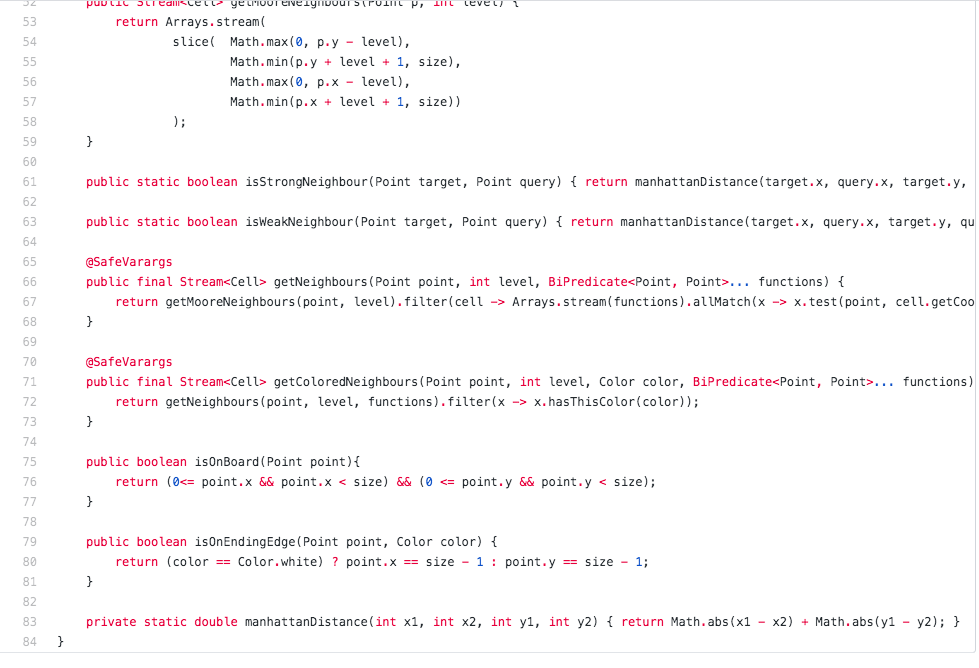
\includegraphics[width=0.5\textwidth]{img/Board.png}}
        \fcolorbox{black}{yellow!70!black!40}

        \vspace{3em}

        \textbf{Board} class was doing too much, so we performed a \textbf{refactor}...

     \end{frame}


     \begin{frame} {Neighbourhood}

     ...and created the \textbf{Neighbourhood} class. It shows a \textbf{Monostate Pattern}, having only static methods to compute different flavours of neighbourhoods from an instance of \textbf{Board} and a target \textbf{Point}.

     \end{frame}


     \begin{frame} {Building Blocks Cont.}

     \textbf{StatusSupervisor} is in charge of holding the state of the game, and updating it whenever it changes (new move, pass rule, pie rule).

     \vspace{1em}

     It is employed as an interface between the \textbf{UI} module and the \textbf{core} module, allowing the two to communicate without knowing anything of each other.

     \end{frame}

     \begin{frame} {Rules}
     The package \textbf{Rules} contains the true logic of the game. We started off by defining a class per rule, later to realize there was room for abstraction...

  	\vspace{1em}

     ...we introduced \textbf{StatusSupervisor} as a \textbf{parameter object}, and allowed each of the classes to implement the \textbf{Rule} interface.

     \vspace{1em}

     Each \textbf{Rule} can be queried by passing a \textbf{Supplier} for it to the \textbf{Rulebook}.

     \end{frame}


     \begin{frame} {Rules Cont.}
     \textbf{ValidPositionRule} class had something wrong...

     \vspace{1em}

     {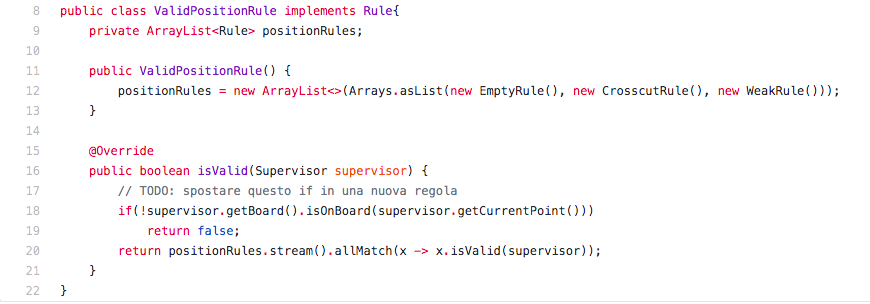
\includegraphics[width=0.5\textwidth]{img/validpositionrule.png}}
        \fcolorbox{black}{yellow!70!black!40}\pause
     {
\includegraphics[width=0.45\textwidth]{img/openclosedprinciple.jpeg}}
     \fcolorbox{black}{yellow!70!black!40}\pause

     \vspace{1em}

     Violation was solved creating \textbf{ValidPositionRulesFactory} class, which follows the \textbf{Factory Pattern}.

     \end{frame}


\section{UI Package}

    %TODO: menzionare i due main?
    %TODO: come interagisce il core con console/GUI?


  \begin{frame}[fragile]{Starting game}

    The console version of the game can be started using:

    \begin{lstlisting}
 > ./gradlew runConsole
    \end{lstlisting}

    \vspace{3em}

    The GUI version of the game can be started using:

    \begin{lstlisting} 
 > ./gradlew runGUI
    \end{lstlisting}

  \end{frame}



  \begin{frame}{Console User Interface}

    \begin{itemize}
      \setlength\itemsep{1em}
      \item \texttt{ConsoleBoardWriter}: board display;
      \item \texttt{ConsoleCellRepresentation}: conversion between cell color and its representation;
      \item \texttt{ConsoleInputHandler}: player input handling;
      \item \texttt{ConsoleMessageWriter}: messages to the players.
    \end{itemize}

    \vspace{1em}

    Messages are contained in the \texttt{Messages} class: its messages are used by the GUI implementation as well.

    %TODO: aggiungere imagine della console.

  \end{frame}



  \begin{frame}{Graphical User Interface}

    \begin{itemize}
      \setlength\itemsep{1em}
      \item \texttt{GUI}: implements the game flow in a \texttt{JavaFX} application;
      \item \texttt{GUIBoardWriter}: board and GUI display;
      \item \texttt{GUIAsker}: \textcolor{red}{boh};
      \item \texttt{GUIMessageWriter}: messages to the players.
    \end{itemize}

    \vspace{1em}

    The \texttt{Events} package defines events for the rules (PieRule, PassRule and EndGameRule); the events are processed by the \texttt{Handlers} package, which handles mouse inputs as well.

    %TODO: aggiungere imagine della GUI.

  \end{frame}


\end{document}
